\documentclass[12pt]{article}
\usepackage[english]{babel}
\usepackage[utf8x]{inputenc}

\usepackage{listings}
\usepackage{xcolor}
\usepackage[landscape]{geometry}

\usepackage{graphicx}
\graphicspath{ {./images/} }

%New colors defined below
\definecolor{codegreen}{rgb}{0,0.6,0}
\definecolor{codegray}{rgb}{0.5,0.5,0.5}
\definecolor{codepurple}{rgb}{0.58,0,0.82}
\definecolor{backcolour}{rgb}{0.95,0.95,0.92}

%Code listing style named "mystyle"
\lstdefinestyle{mystyle}{
  backgroundcolor=\color{backcolour},   
  commentstyle=\color{codegreen},
  keywordstyle=\color{magenta},
  numberstyle=\tiny\color{codegray},
  stringstyle=\color{codepurple},
  basicstyle=\ttfamily\footnotesize,
  breakatwhitespace=false,         
  breaklines=true,                 
  captionpos=b,                    
  keepspaces=true,                 
  numbers=left,                    
  numbersep=5pt,                  
  showspaces=false,                
  showstringspaces=false,
  showtabs=false,                  
  tabsize=2
}

%"mystyle" code listing set
\lstset{style=mystyle}


\begin{document}

%\section{Plots}
% 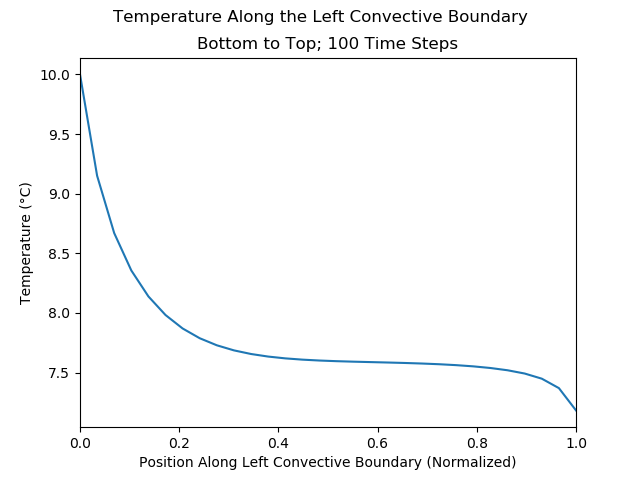
\includegraphics[width=\textwidth]{Problem-Set-6-Figure-1.png}
% \clearpage
% 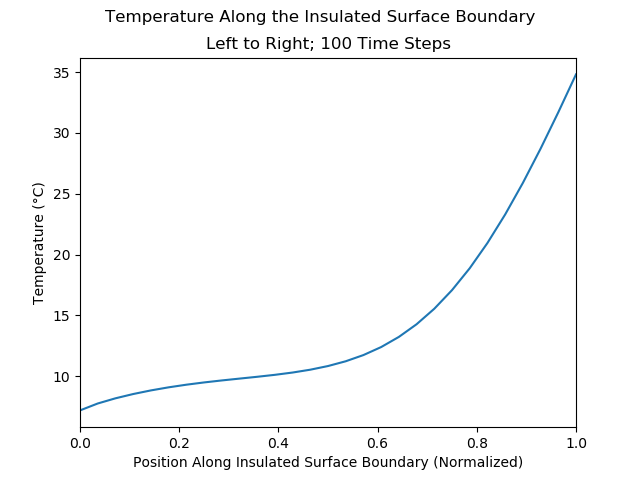
\includegraphics[width=\textwidth]{Problem-Set-6-Figure-2.png}
% \clearpage
% 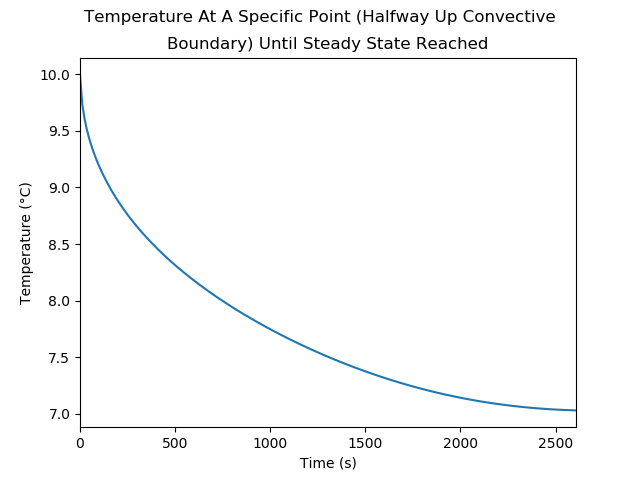
\includegraphics[width=\textwidth]{Problem-Set-6-Figure-3.png}
% \clearpage
% 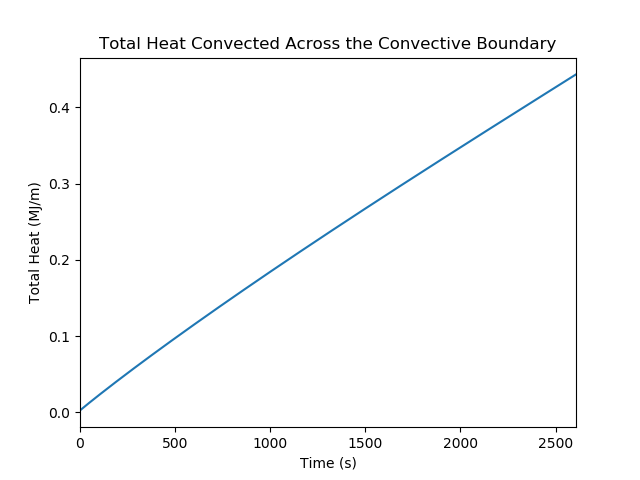
\includegraphics[width=\textwidth]{Problem-Set-6-Figure-4.png}
% \clearpage
% \includegraphics[width=\textwidth]{Problem-Set-56Figure-5.png}
% \clearpage

\section{PSet-6.py}
\lstinputlisting[language=Python]{PSet-6.py}

\end{document}